\documentclass[12pt]{article}
\usepackage{ucs}
\usepackage[utf8x]{inputenc}
\usepackage[turkish,english]{babel}
\usepackage{graphicx}
\usepackage{url}
\usepackage[sc]{mathpazo}
\linespread{1.05}
\usepackage[T1]{fontenc}
\usepackage[a2paper,margin=1cm]{geometry}
\usepackage{shapepar}
\pagestyle{empty}

\author{Mehmet Atakan Gürkan}
\title{}
\date{}
\newcommand\almleftshape{
   {0}
   {0}b{0}
\\ {0}t{0}{7}
\\ {17}t{0}{11.5}
\\ {19}t{0}{11.7}
\\ {21}t{0}{11.7}
\\ {24}t{0}{11.3}
\\ {34}t{0}{8.3}
\\ {41}t{0}{4.4}
\\ {42}e{0}}
\newcommand\almrightshape{
   {12}
   {0}b{0}
\\ {0}t{3.2}{6.8}
\\ {1}t{4}{6}
\\ {5}t{2.6}{7.4}
\\ {10}t{1.0}{9}
\\ {15}t{-0.6}{10.6}
\\ {17}t{-1}{11.0}
\\ {19}t{-1.2}{11.2}
\\ {21}t{-1}{11.0}
\\ {27}t{0}{10.0}
\\ {41}t{3.5}{6.5}
\\ {42}e{10}}
\begin{document}
%\maketitle
\shorthandoff{=}
\centerline{\raisebox{-24pt}{
\includegraphics[clip,height=72pt]{logo2}}
     \fontsize{40pt}{40pt}\selectfont
     \,için Gökyüzü Almanağı / Sky Almanac for\,
\raisebox{-24pt}{
\includegraphics[clip,height=72pt]{logo2}}}
\vskip 2cm
\noindent
\centerline{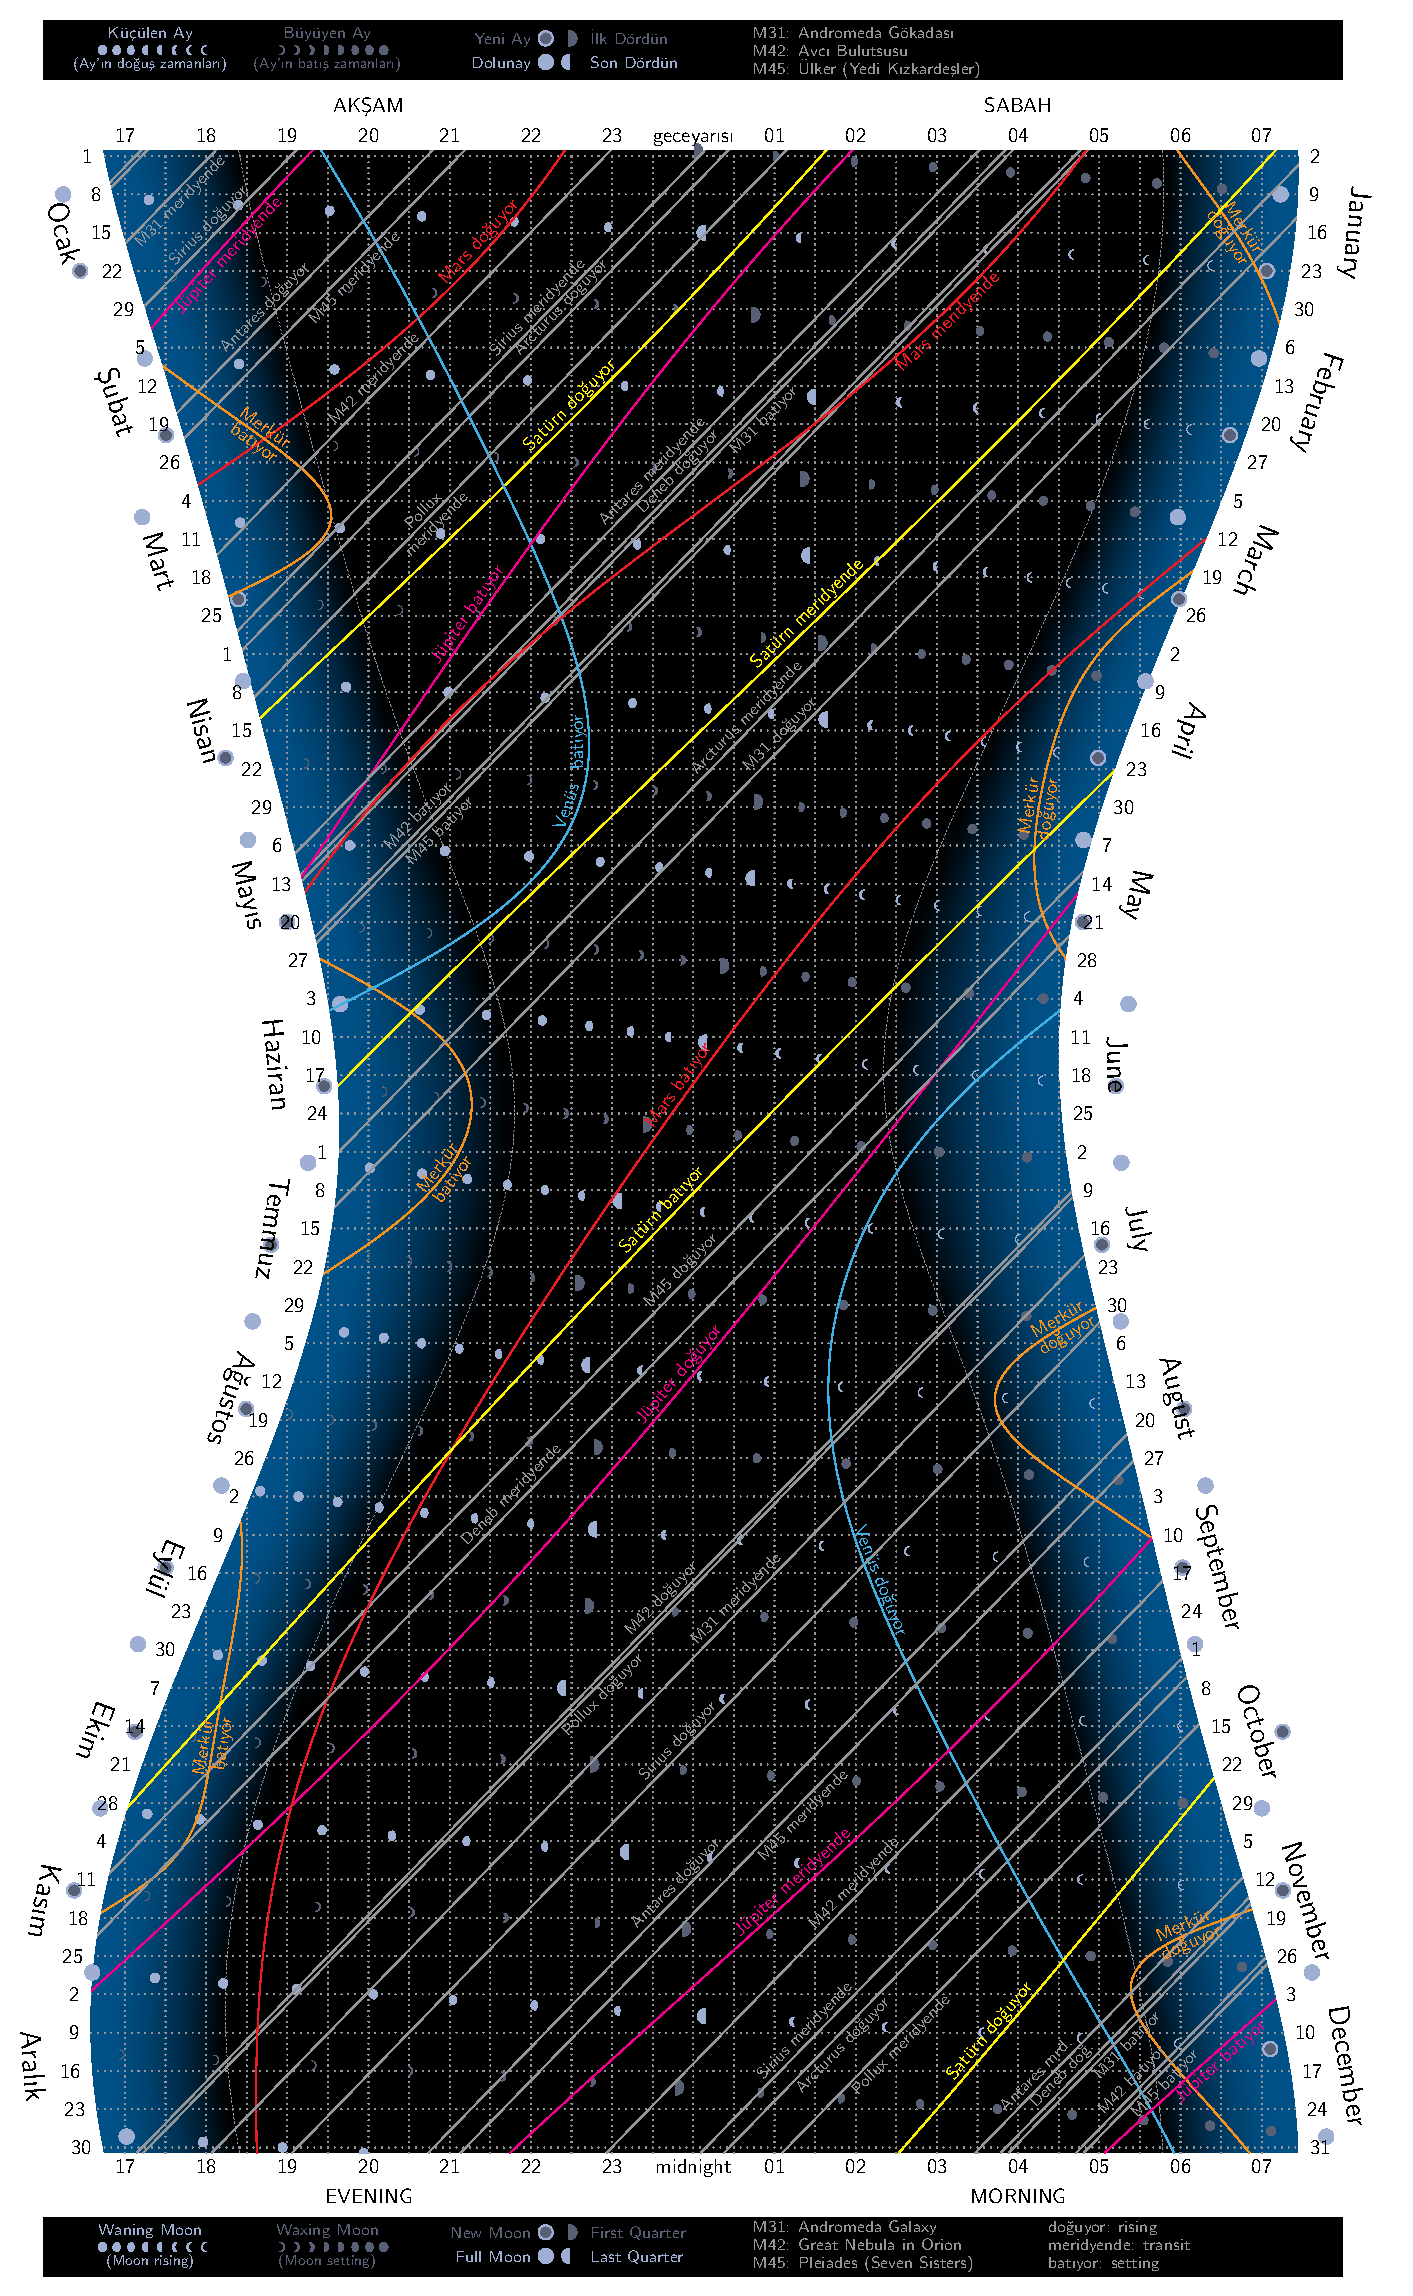
\includegraphics[clip,height=0.9\textheight]{almanac_2012_SabanciUniv}}

\vskip -0.9\textheight \vskip9cm
\noindent
\cutout{l}(0cm,0pt)
\shapepar{\almleftshape}{\fontsize{13pt}{13pt}\selectfont
\selectlanguage{turkish}
\hskip0.4cm\textbf{Çizelgenin Kullanımı}\\
Bu çizelge 2012 yılı için Sabancı Üniversitesi'nde çeşitli
gök cisimlerinin doğma, meridyenden (gökyüzünde ulaştıkları en
yüksek noktadan) geçme ve batma zamanlarını, alacakaranlığın
sonuyla başlangıcını ve Ay'ın evrelerini veriyor.  Dikey eksen
günleri, yatay eksen gece boyunca zamanı gösteriyor.  Gece içinde
yarımşar saatlik aralıklar ve yıl içinde Pazar akşamlarını
Pazartesi sabahlarına bağlayan geceler noktalı çizgilerle
belirtiliyor. Düşey olarak iki nokta arası bir güne, yatay olarak
iki nokta arası beş dakikaya karşılık geliyor.\\
Bir örnek olarak 9 Mart gecesinin olaylarına bakarsak: İlk olarak,
sol tarafta 11 Mart'a karşılık gelen noktanın üstünde yaklaşık
olarak 13 Mart'a karşılık gelen noktayı bulmak gerekiyor. Buradan
sağa doğru ilerlediğimizde 18:30 civarında Avcı Bulutsusu'nun
meridyenden geçeceğini görüyoruz. Bunun ardından 19:30'da
Merkür batıyor, 19:45 civarında Sirius meridyenden geçiyor ve
20:00 civarında Arcturus doğuyor. Bu bilgilerden Güneş battığı
zaman Orion Bulutsusu, Merkür ve Sirius'un ufkun üzerinde olduğunu
da anlıyoruz. Sağa doğru ilerledikçe, belli saatlerde pekçok
gökcisminin doğduğunu, meridyenden geçtiğini ve battığını
görüyoruz. 19:40 civarında gördüğümüz Ay sembolü, Ay'ın
doğuş zamanını gösteriyor ve bir sonraki gece Ay'ın daha
küçük olacağını belirtiyor. Son olarak 19:35 ve 4:50 civarında
gördüğümüz kesikli çizgiler sırasıyla alacakaranlığın
bitmesi ve başlamasını belirtiyor. Bu noktalar Güneş'in ufkun
18$^\circ$ altında kaldığı anlara karşılık geliyor.\\
Çizelgede verilen doğma ve batma zamanları, ufuk çizgisinin önünde bir engel
olmadığını varsayıyor. Eğer böyle bir engel varsa, her bir
açı derecesi yükseklik için doğma zamanı 4 dakika geç, batma zamanı da
aynı miktarda erken olacak. Benzer biçimde, yüksek bir noktadan gözlem
yapıldığı için ufuk çizgisi olması gerekenin altında ise, doğma ve batma
zamanlarının düzeltilmesi gerekecek.\\
Not: Yaz saati uygulamasının olduğu zamanlarda,
çizelgedeki zamanlara
bir saat eklemek gerekiyor.\\
~}
\vskip -6.7cm
\cutout{r}(2em,6cm)
\shapepar{\almrightshape}{\fontsize{13pt}{13pt}\selectfont
\selectlanguage{english}
\hskip 1.2cm\textbf{Using the Chart}\\
This chart gives the rise, transit (reaching the highest point in
the sky) and setting time for various stellar objects, the end and the
beginning of the twilight, and the phases of the Moon for Sabancı
University in the year 2012. The vertical axis denotes the days and
the horizontal axis denotes the time through the night. Every half
hour during the night and the nights of Sunday evenings and Monday
mornings are indicated by dotted lines.  In the vertical lines, each
point corresponds to a day; and for the horizontal lines to five minutes. \\
As an example, let's look at the night of March 9$^\textrm{th}$:
First of all, we need to find the point corresponding to March 9, just
above March 11 mark. As we proceed to the right from this point,
we see that Orion Nebula transits around 18:30. This is followed by
    Mercury setting at about 19:30, Sirius transiting around 19:45 and
Arcturus rising around 20:00. From this, we also gather that Orion
Nebula, Mercury and Sirius were on the sky as the Sun set.
As we go further right, we see more objects rising, transitting and
setting. The Moon symbol that we see around 19:40, indicates the rising
time of a waning moon (Moon will get smaller the next night). Finally,
the dashed lines around 19:35 and 4:50 indicate the end of the evening
twilight and the beginning of the morning twilight. These points are
determined by calculating the time that Sun is 18$^\circ$ below
horizon.\\
The rise and set times in the chart are calculated by assuming that
there is no obstacle in front of the horizon. If there is such an
obstacle, for each degree angle of its height rising time will be 4
minutes late and setting time 4 minutes early. Likewise, if the horizon
is below horizontal, an adjustment has to be made.\\
PS: While daylight savings time (a.k.a. summer time) is in effect,
you need to add one hour to the times given in the chart.\\ ~}
\vskip 48.5cm \footnotesize

{\hfill M. Atakan Gürkan \url{<agurkan@sabanciuniv.edu>}}

{\hfill \url{https://github.com/atakan/PySkyAlmanac/sabanci}}
\end{document}
